\documentclass[crop,tikz]{standalone}% 'crop' is the default for v1.0, before it was 'preview'
\usepackage{tikz,calc,pgfplots}
\usetikzlibrary{calc}
\begin{document}
	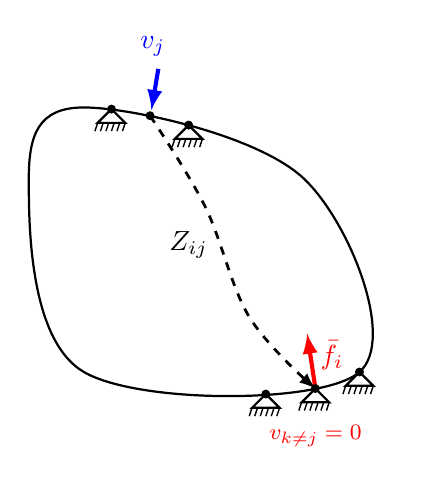
\begin{tikzpicture}[scale = 0.7]
		
		%	
		%	\draw [thick]  plot[smooth cycle, tension=.6] coordinates {(0,2) (0.5,4.5) (4,5.2) (6,4.5)  (5.35,2.5) (5.5,0.85) (4,0) (1,0.5) };
		%	\node[outer sep=0pt,thick] at (5.2,4.2) [] {${A}$};
		
		
		
		\draw [thick]  plot[smooth cycle, tension=.6] coordinates {(0,-1) (1,-4.5) (6,-4.5) (5,-1) (1,0.3) };
		
		
		
		\draw[black,fill=black] (2.9,-0.02) circle (2pt);
			\begin{scope}[xshift=2.9cm,yshift=-0.02cm]
				\draw [thick]  plot[] coordinates {(0,0) (0.25,-0.25) (-0.25, -0.25) (0,0) };
				\draw [line width=0.5pt]  (-0.25,-0.25) -- ++( -0.05, -0.15) ; 
				\draw [line width=0.5pt]  (-0.15,-0.25) -- ++( -0.05, -0.15) ; 
				\draw [line width=0.5pt]  (-0.05,-0.25) -- ++( -0.05, -0.15) ; 
				\draw [line width=0.5pt]  (0.05,-0.25) -- ++( -0.05, -0.15) ; 
				\draw [line width=0.5pt]  (0.15,-0.25) -- ++( -0.05, -0.15) ; 
				\draw [line width=0.5pt]  (0.25,-0.25) -- ++( -0.05, -0.15) ; 
			\end{scope}
		
		\draw[black,fill=black] (2.2,0.15) circle (2pt);

		
		\draw[black,fill=black] (1.5,0.27) circle (2pt);
					\begin{scope}[xshift=1.5cm,yshift=0.27cm]
			\draw [thick]  plot[] coordinates {(0,0) (0.25,-0.25) (-0.25, -0.25) (0,0) };
			\draw [line width=0.5pt]  (-0.25,-0.25) -- ++( -0.05, -0.15) ; 
			\draw [line width=0.5pt]  (-0.15,-0.25) -- ++( -0.05, -0.15) ; 
			\draw [line width=0.5pt]  (-0.05,-0.25) -- ++( -0.05, -0.15) ; 
			\draw [line width=0.5pt]  (0.05,-0.25) -- ++( -0.05, -0.15) ; 
			\draw [line width=0.5pt]  (0.15,-0.25) -- ++( -0.05, -0.15) ; 
			\draw [line width=0.5pt]  (0.25,-0.25) -- ++( -0.05, -0.15) ; 
		\end{scope}
	
		\draw [line width=1.5pt,blue,latex-]  plot[smooth, tension=.6] coordinates {(2.225,0.25)  (2.35,1) }; 
		\node[outer sep=0pt,thick] at (2.25,1.4) [] {{\color{blue}${{v}}_{j}$}};
		
		\draw [line width=1.5pt,red,-latex]  (5.2,-4.8) -- ++( -0.15, 1)  ;
		\node[outer sep=0pt,thick] at (5.5,-4.2) [] {{\color{red}${\bar{f}}_{i}$}};
		
		
		\draw [line width=1pt,dashed,-latex]  plot[smooth, tension=.6] coordinates {(2.2,0.15) (3.2,-1.5) (4,-3.5)  (5.2,-4.8) }; 
		\node[outer sep=0pt,thick] at (2.9,-2.2) [] {{${Z}_{ij}$}};
		
		\draw[black,fill=black] (6,-4.5) circle (2pt);
		\draw[black,fill=black] (5.2,-4.8) circle (2pt);
		\draw[black,fill=black] (4.3,-4.9) circle (2pt);
		
		\begin{scope}[xshift=4.3cm,yshift=-4.9cm]
			\draw [thick]  plot[] coordinates {(0,0) (0.25,-0.25) (-0.25, -0.25) (0,0) };
			\draw [line width=0.5pt]  (-0.25,-0.25) -- ++( -0.05, -0.15) ; 
			\draw [line width=0.5pt]  (-0.15,-0.25) -- ++( -0.05, -0.15) ; 
			\draw [line width=0.5pt]  (-0.05,-0.25) -- ++( -0.05, -0.15) ; 
			\draw [line width=0.5pt]  (0.05,-0.25) -- ++( -0.05, -0.15) ; 
			\draw [line width=0.5pt]  (0.15,-0.25) -- ++( -0.05, -0.15) ; 
			\draw [line width=0.5pt]  (0.25,-0.25) -- ++( -0.05, -0.15) ; 
		\end{scope}
		
		\begin{scope}[xshift=5.2cm,yshift=-4.8cm]
			\draw [thick]  plot[] coordinates {(0,0) (0.25,-0.25) (-0.25, -0.25) (0,0) };
			\draw [line width=0.5pt]  (-0.25,-0.25) -- ++( -0.05, -0.15) ; 
			\draw [line width=0.5pt]  (-0.15,-0.25) -- ++( -0.05, -0.15) ; 
			\draw [line width=0.5pt]  (-0.05,-0.25) -- ++( -0.05, -0.15) ; 
			\draw [line width=0.5pt]  (0.05,-0.25) -- ++( -0.05, -0.15) ; 
			\draw [line width=0.5pt]  (0.15,-0.25) -- ++( -0.05, -0.15) ; 
			\draw [line width=0.5pt]  (0.25,-0.25) -- ++( -0.05, -0.15) ; 
			\node[outer sep=0pt,thick] at (0, 0)  [yshift=-0.6cm] {\footnotesize{\color{red}$v_{k\neq j}=0$}};
		\end{scope}
		
		\begin{scope}[xshift=6cm,yshift=-4.5cm]
			\draw [thick]  plot[] coordinates {(0,0) (0.25,-0.25) (-0.25, -0.25) (0,0) };
			\draw [line width=0.5pt]  (-0.25,-0.25) -- ++( -0.05, -0.15) ; 
			\draw [line width=0.5pt]  (-0.15,-0.25) -- ++( -0.05, -0.15) ; 
			\draw [line width=0.5pt]  (-0.05,-0.25) -- ++( -0.05, -0.15) ; 
			\draw [line width=0.5pt]  (0.05,-0.25) -- ++( -0.05, -0.15) ; 
			\draw [line width=0.5pt]  (0.15,-0.25) -- ++( -0.05, -0.15) ; 
			\draw [line width=0.5pt]  (0.25,-0.25) -- ++( -0.05, -0.15) ; 
			% \node[outer sep=0pt,thick] at (0, 0)  [yshift=-0.4cm] {\footnotesize{\color{red}$v=0$}};
		\end{scope}
		
		
		
	\end{tikzpicture}
\end{document}